\documentclass[tikz,border=2mm]{standalone}

\begin{document}

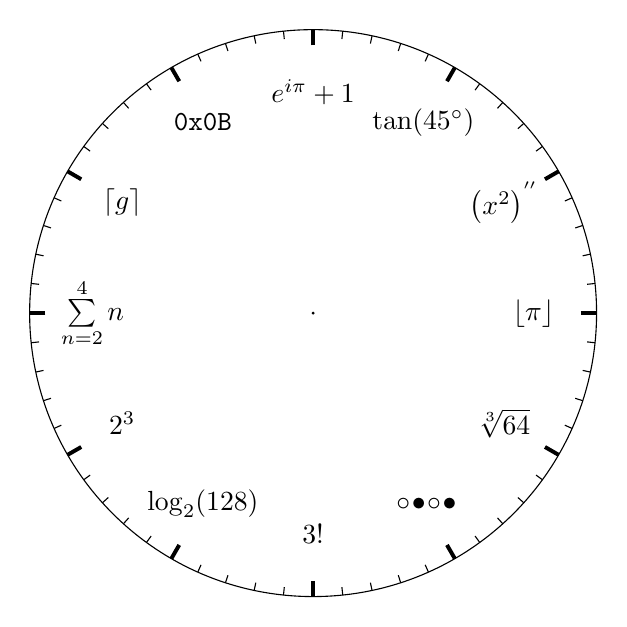
\begin{tikzpicture}
	\draw[fill] (0,0) circle (.1mm);
	\draw (0,0) circle (3.6cm);
	
	\foreach \angle in {6,12,...,360}
		\draw (-\angle:3.5cm) -- ++(-\angle:.1cm);

	\foreach \hour / \label in {
		1/$\tan(45^\circ)$,
		2/$\left(x^2\right)^{''}$,
		3/$\lfloor \mathbf{\pi} \rfloor$,
		4/$\sqrt[3]{64}$,
		5/${}\circ\!\bullet\!\circ\!\bullet$,
		6/$3!$,
		7/$\log_2({128})$,
		8/$2^3$,
		9/$\sum\limits_{n=2}^4n$,
		10/$\lceil g \rceil$,
		11/\texttt{0x0B},
		12/$e^{i\pi}+1$
	}{
		\def\angle{\hour*360/12+90}
		\node at (-\angle:2.8cm) {\label};
		\draw[line width=.5mm] (-\angle:3.4cm) -- ++(-\angle:.2cm);
	}
\end{tikzpicture}

\end{document}
